% 2-15-rb-tree.tex

%%%%%%%%%%%%%%%%%%%%
\documentclass[a4paper, justified]{tufte-handout}

% hw-preamble.tex

% geometry for A4 paper
% See https://tex.stackexchange.com/a/119912/23098
\geometry{
  left=20.0mm,
  top=20.0mm,
  bottom=20.0mm,
  textwidth=130mm, % main text block
  marginparsep=5.0mm, % gutter between main text block and margin notes
  marginparwidth=50.0mm % width of margin notes
}

% for colors
\usepackage{xcolor} % usage: \color{red}{text}
% predefined colors
\newcommand{\red}[1]{\textcolor{red}{#1}} % usage: \red{text}
\newcommand{\blue}[1]{\textcolor{blue}{#1}}
\newcommand{\teal}[1]{\textcolor{teal}{#1}}

\usepackage{todonotes}

% heading
\usepackage{sectsty}
\setcounter{secnumdepth}{2}
\allsectionsfont{\centering\huge\rmfamily}

% for Chinese
\usepackage{xeCJK}
\usepackage{zhnumber}
\setCJKmainfont[BoldFont=FandolSong-Bold.otf]{FandolSong-Regular.otf}

% for fonts
\usepackage{fontspec}
\newcommand{\song}{\CJKfamily{song}} 
\newcommand{\kai}{\CJKfamily{kai}} 

% To fix the ``MakeTextLowerCase'' bug:
% See https://github.com/Tufte-LaTeX/tufte-latex/issues/64#issuecomment-78572017
% Set up the spacing using fontspec features
\renewcommand\allcapsspacing[1]{{\addfontfeature{LetterSpace=15}#1}}
\renewcommand\smallcapsspacing[1]{{\addfontfeature{LetterSpace=10}#1}}

% for url
\usepackage{hyperref}
\hypersetup{colorlinks = true, 
  linkcolor = teal,
  urlcolor  = teal,
  citecolor = blue,
  anchorcolor = blue}

\newcommand{\me}[4]{
    \author{
      {\bfseries 姓名:}\underline{#1}\hspace{2em}
      {\bfseries 学号:}\underline{#2}\hspace{2em}\\[10pt]
      {\bfseries 评分:}\underline{#3\hspace{3em}}\hspace{2em}
      {\bfseries 评阅:}\underline{#4\hspace{3em}}
  }
}

% Please ALWAYS Keep This.
\newcommand{\noplagiarism}{
  \begin{center}
    \fbox{\begin{tabular}{@{}c@{}}
      请独立完成作业,不得抄袭。\\
      若得到他人帮助, 请致谢。\\
      若参考了其它资料,请给出引用。\\
      鼓励讨论,但需独立书写解题过程。
    \end{tabular}}
  \end{center}
}

\newcommand{\goal}[1]{
  \begin{center}{\fcolorbox{blue}{yellow!60}{\parbox{0.50\textwidth}{\large 
    \begin{itemize}
      \item 体会``思维的乐趣''
      \item 初步了解递归与数学归纳法 
      \item 初步接触算法概念与问题下界概念
    \end{itemize}}}}
  \end{center}
}

% Each hw consists of four parts:
\newcommand{\beginrequired}{\hspace{5em}\section{作业 (必做部分)}}
\newcommand{\beginoptional}{\section{作业 (选做部分)}}
\newcommand{\beginot}{\section{Open Topics}}
\newcommand{\begincorrection}{\section{订正}}
\newcommand{\beginfb}{\section{反馈}}

% for math
\usepackage{amsmath, mathtools, amsfonts, amssymb}
\newcommand{\set}[1]{\{#1\}}

% define theorem-like environments
\usepackage[amsmath, thmmarks]{ntheorem}

\theoremstyle{break}
\theorempreskip{2.0\topsep}
\theorembodyfont{\song}
\theoremseparator{}
\newtheorem{problem}{题目}[subsection]
\renewcommand{\theproblem}{\arabic{problem}}
\newtheorem{ot}{Open Topics}

\theorempreskip{3.0\topsep}
\theoremheaderfont{\kai\bfseries}
\theoremseparator{:}
\theorempostwork{\bigskip\hrule}
\newtheorem*{solution}{解答}
\theorempostwork{\bigskip\hrule}
\newtheorem*{revision}{订正}

\theoremstyle{plain}
\newtheorem*{cause}{错因分析}
\newtheorem*{remark}{注}

\theoremstyle{break}
\theorempostwork{\bigskip\hrule}
\theoremsymbol{\ensuremath{\Box}}
\newtheorem*{proof}{证明}

% \newcommand{\ot}{\blue{\bf [OT]}}

% for figs
\renewcommand\figurename{图}
\renewcommand\tablename{表}

% for fig without caption: #1: width/size; #2: fig file
\newcommand{\fig}[2]{
  \begin{figure}[htbp]
    \centering
    \includegraphics[#1]{#2}
  \end{figure}
}
% for fig with caption: #1: width/size; #2: fig file; #3: caption
\newcommand{\figcap}[3]{
  \begin{figure}[htbp]
    \centering
    \includegraphics[#1]{#2}
    \caption{#3}
  \end{figure}
}
% for fig with both caption and label: #1: width/size; #2: fig file; #3: caption; #4: label
\newcommand{\figcaplbl}[4]{
  \begin{figure}[htbp]
    \centering
    \includegraphics[#1]{#2}
    \caption{#3}
    \label{#4}
  \end{figure}
}
% for margin fig without caption: #1: width/size; #2: fig file
\newcommand{\mfig}[2]{
  \begin{marginfigure}
    \centering
    \includegraphics[#1]{#2}
  \end{marginfigure}
}
% for margin fig with caption: #1: width/size; #2: fig file; #3: caption
\newcommand{\mfigcap}[3]{
  \begin{marginfigure}
    \centering
    \includegraphics[#1]{#2}
    \caption{#3}
  \end{marginfigure}
}

\usepackage{fancyvrb}

% for algorithms
\usepackage[]{algorithm}
\usepackage[]{algpseudocode} % noend
% See [Adjust the indentation whithin the algorithmicx-package when a line is broken](https://tex.stackexchange.com/a/68540/23098)
\newcommand{\algparbox}[1]{\parbox[t]{\dimexpr\linewidth-\algorithmicindent}{#1\strut}}
\newcommand{\hStatex}[0]{\vspace{5pt}}
\makeatletter
\newlength{\trianglerightwidth}
\settowidth{\trianglerightwidth}{$\triangleright$~}
\algnewcommand{\LineComment}[1]{\Statex \hskip\ALG@thistlm \(\triangleright\) #1}
\algnewcommand{\LineCommentCont}[1]{\Statex \hskip\ALG@thistlm%
  \parbox[t]{\dimexpr\linewidth-\ALG@thistlm}{\hangindent=\trianglerightwidth \hangafter=1 \strut$\triangleright$ #1\strut}}
\makeatother

% for footnote/marginnote
% see https://tex.stackexchange.com/a/133265/23098
\usepackage{tikz}
\newcommand{\circled}[1]{%
  \tikz[baseline=(char.base)]
  \node [draw, circle, inner sep = 0.5pt, font = \tiny, minimum size = 8pt] (char) {#1};
}
\renewcommand\thefootnote{\protect\circled{\arabic{footnote}}} % feel free to modify this file
%%%%%%%%%%%%%%%%%%%%
\title{第4-4讲: 数论初步}
\me{朱宇博 }{191220186 }{}{}
\date{\zhtoday} % or like 2019年9月13日
%%%%%%%%%%%%%%%%%%%%
\begin{document}
\maketitle
%%%%%%%%%%%%%%%%%%%%
\noplagiarism % always keep this line
%%%%%%%%%%%%%%%%%%%%
\begin{abstract}
  % \begin{center}{\fcolorbox{blue}{yellow!60}{\parbox{0.65\textwidth}{\large 
  %   \begin{itemize}
  %     \item 
  %   \end{itemize}}}}
  % \end{center}
\end{abstract}
%%%%%%%%%%%%%%%%%%%%
\beginrequired

%%%%%%%%%%%%%%%
\begin{problem}[TJ 2-15(b,f)]
For each of the following pairs of numbers a and b, calculate gcd(a,b) and find integers r and s such that gcd(a, b) = ra + sb.\\
(b)234 and 165\\
(f)−4357 and 3754\\
\end{problem}

\begin{solution}
(b)\\
\[
\begin{aligned}
234&=165\times 1 + 69\\
165&=69\times 2 + 27\\
69 & = 27\times 2 + 15\\
27 & = 15\times 1 + 12\\
15& = 12\times 1 + 3\\
12 & = 3 \times 4 + 0\\
\end{aligned}
\]
Therefore gcd(234, 165) = 3\\
\[
\begin{aligned}
3 &= 1\times15 + (-1)\times 12\\
&=(-1)\times27 + 2\times 15\\
&=2\times 69 + (-5)\times 27\\
&=12\times 69 + (-5)\times 165\\
&=2\times 69 + (-5)\times 27\\
&=12\times 234 + (-17)\times 165\\
\end{aligned}
\]
So $r=12,s=-17$\\
\newpage
\noindent(f)\\
\[
\begin{aligned}
-4357&=3754\times(-1) + (-603)\\
3754&= (-603)\times (-6) + 136\\
-603 &=136\times (-4) + (-59)\\
136 &=(-59)\times(-2) + 18\\
-59 & = 18\times (-3) + (-5)\\
18 & = (-5)\times(-3) + (-3)\\
-5 &=(-3)\times1 + (-2)\\
(-3) & = (-2)\times 1 + (-1)\\
(-2) & = (-1)\times2 + 0 
\end{aligned}
\]
Therefore gcd(−4357, 3754) = 1\\
 \begin{figure}[htbp]
    \centering
    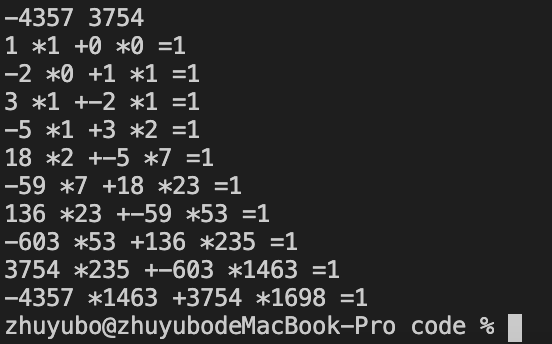
\includegraphics[width = 0.60\linewidth]{figs/a}
  \end{figure}

So $r=1463,s=1698$\\

\end{solution}
%%%%%%%%%%%%%%%

%%%%%%%%%%%%%%%
\begin{problem}[TJ 2-16]
Let $a$ and $b$ be nonzero integers. If there exist integers $r$ and $s$ such that $ar + bs = 1$, show that a and b are relatively prime.
\end{problem}

\begin{solution}
由Theorem 2.10的证明过程可知,$S=\{am+bn:m,n\in\mathbb{Z} \land am + bn >0\}$中的最小元是gcd(a,b)。\\
由集合$S$的性质,显然有:若$1\in S$,则1为S中最小元,即为gcd(a,b)\\
由题设可知$1$在集合$S$中。故gcd(a,b)=1, a和b互质
\end{solution}
%%%%%%%%%%%%%%%

%%%%%%%%%%%%%%%
\begin{problem}[TJ 2-19]
Let $x,y \in N$ be relatively prime. If $xy$ is a perfect square, prove that x and y must
both be perfect squares.
\end{problem}

\begin{solution}
反证法。假设$x$不为完全平方数,则$x$存在一个质因子$a$,在$x$的质数乘积分解中,出现奇数次。\\
由于$x,y$互质,则在$y$的质数乘积分解中,不会出现质因子$a$。\\
故在$xy$的的质数乘积分解中,质因子$a$出现的次数仍为奇数次,故$xy$不为完全平方数,与题设矛盾。\\
得证
\end{solution}
%%%%%%%%%%%%%%%

%%%%%%%%%%%%%%%
\begin{problem}[TJ 2-29]
Prove that there are an infinite number of primes of the form 6n + 5.
\end{problem}

\begin{solution}
反证。假设$S=\{x | x \quad is \quad prime  \land \exists p, 6p+5 = x\}$为有限集,记$|S|=N$\\
令$T=\prod \limits_{i=1}^{N}x_i$, $x_i\in S$。\\
当$N$为奇数时,$T$模6为5,故$T+6$模6为5。\\
在$T+6$的所有质因子中,一定存在形如$6n+5$的质因子。否则,$T+6$模6不为5。\\
由于$x_i(x_i\in S)$都不为$T+6$的因子,则存在一个形如$6n+5$的质数,不在集合$S$中,与假设矛盾。\\
当$N$为偶数时,$T$模6为1,故$T+4$模6为5。\\
在$T+4$的所有质因子中,一定存在形如$6n+5$的质因子。否则,$T+4$模6不为5。\\
由于$x_i(x_i\in S)$都不为$T+4$的因子,则存在一个形如$6n+5$的质数,不在集合$S$中,与假设矛盾。\\
故形如$6n+5$的质数有无穷多个。
\end{solution}
%%%%%%%%%%%%%%%

%%%%%%%%%%%%%%%
\begin{problem}[TJ 2-30]
Prove that there are an infinite number of primes of the form 4n − 1.
\end{problem}

\begin{solution}
反证。假设$S=\{x | x \quad is \quad prime  \land \exists p, 4n-1 = x\}$为有限集,记$|S|=N$\\
令$T=\prod \limits_{i=1}^{N}x_i$, $x_i\in S$。\\
当$N$为奇数时,$T$模4为3,故$T+4$模4为3。\\
在$T+4$的所有质因子中,一定存在形如$4n-1$的质因子。否则,$T+4$模4不为3。\\
由于$x_i(x_i\in S)$都不为$T+4$的因子,则存在一个形如$4n-1$的质数,不在集合$S$中,与假设矛盾。\\
当$N$为偶数时,$T$模4为1,故$T+2$模4为3。\\
在$T+2$的所有质因子中,一定存在形如$4n-1$的质因子。否则,$T+2$模4不为3。\\
由于$x_i(x_i\in S)$都不为$T+2$的因子,则存在一个形如$4n-1$的质数,不在集合$S$中,与假设矛盾。\\
故形如$4n-1$的质数有无穷多个。
\end{solution}
%%%%%%%%%%%%%%%

%%%%%%%%%%%%%%%
\begin{problem}[CS 2.2-2]
If a·133−m·277 = 1, does this guarantee that a has an inverse mod m? If so, what
is it? If not, why not?
\end{problem}

\begin{solution}
存在逆,由a·133−m·277 = 1,我们可知gcd(a,m)=1,且$133a\equiv  1 \pmod m$,故$a$的逆为$133\mod m$
\end{solution}
%%%%%%%%%%%%%%%

%%%%%%%%%%%%%%%
\begin{problem}[CS 2.2-4]
How many elements a are there such that a·$_{31}$22 = 1? How many elements a are
there such that a·$_{10}$2 = 1?
\end{problem}

\begin{solution}
(1)\\
因为gcd(31,22)=1, 故$22$存在一个在模31意义下的逆。数量为1\\
(2)\\
因为$gcd(10,2)\neq1$, 故$2$不存在一个在模10意义下的逆。数量为0\\
\end{solution}
%%%%%%%%%%%%%%%

%%%%%%%%%%%%%%%
\begin{problem}[CS 2.2-6]
If a·133−m·277 = 1, what can you say about all possible common divisors of a and
m?
\end{problem}

\begin{solution}
若满足上述等式,则a与m互质,其公因数只有1和-1
\end{solution}
%%%%%%%%%%%%%%%

%%%%%%%%%%%%%%%
\begin{problem}[CS 2.2-8]
If k = jq +r, as in Euclid’s division theorem, is there a relationship between gcd(q, k)
and gcd(r, q)? If so, what is it?
\end{problem}

\begin{solution}
gcd(q, k) =gcd(r, q).\\
其中j和q是等同地位的,可相互替换。\\
由欧几里得定理可得两者最大公因数相同
\end{solution}
%%%%%%%%%%%%%%%

%%%%%%%%%%%%%%%
\begin{problem}[CS 2.2-16]
\end{problem}

\begin{solution}
若m为负数,则存在唯一的$q$和$r$,使得$-m=nq+r$,其中$0\leq r<n$\\
若$r$为0,则显然有m=n(-q)+r 满足该形式。\\
若$r$大于0,因为$-m=nq+r$,则有$m=-nq-r$, 令$q'=-q-1$,则$m=n(q'+1)-r=nq'+(n-r)$\\
此式满足上述形式。\\
以下证明唯一性。假设存在$q$和$r$,$q'$和$r'$满足$m=nq+r$, $m=nq'+r'$, 其中$0\leq r<n$, $0\leq r'<n$\\
因此有$n(q-q')=r'-r$,即$n|r'-r$,由于$0\leq r<n$, $0\leq r'<n$, 故$|r'-r|<n$。因此可推得$r=r'$。\\
所以$n(q-q')=0$,得$q-q'$\\
故唯一性可证
\end{solution}
%%%%%%%%%%%%%%%

%%%%%%%%%%%%%%%
\begin{problem}[CS 2.2-19]
\end{problem}

\begin{solution}
$lcm(x,y)=\frac{xy}{gcd(x,y)}$
\end{solution}
%%%%%%%%%%%%%%%
%%%%%%%%%%%%%%%%%%%%
\beginoptional


%%%%%%%%%%%%%%%%%%%%
\beginot
%%%%%%%%%%%%%%%
\begin{ot}[介绍皮亚诺公理]	

\end{ot}

% \begin{solution}
% \end{solution}
%%%%%%%%%%%%%%%

%%%%%%%%%%%%%%%
\begin{ot}[Miller-Rabin Algorithm]	
\end{ot}


% \begin{solution}
% \end{solution}
%%%%%%%%%%%%%%%


% \vspace{0.50cm}
%%%%%%%%%%%%%%%
% \begin{ot}[]
% 
%   \noindent 参考资料:
%   \begin{itemize}
%     \item 
%   \end{itemize}
% \end{ot}

% \begin{solution}
% \end{solution}
%%%%%%%%%%%%%%%

%%%%%%%%%%%%%%%%%%%%
% 如果没有需要订正的题目,可以把这部分删掉

% \begincorrection
%%%%%%%%%%%%%%%%%%%%

%%%%%%%%%%%%%%%%%%%%
% 如果没有反馈,可以把这部分删掉
\beginfb

% 你可以写
% ~\footnote{优先推荐 \href{problemoverflow.top}{ProblemOverflow}}:
% \begin{itemize}
%   \item 对课程及教师的建议与意见
%   \item 教材中不理解的内容
%   \item 希望深入了解的内容
%   \item $\cdots$
% \end{itemize}
%%%%%%%%%%%%%%%%%%%%
% \bibliography{2-5-solving-recurrence}
% \bibliographystyle{plainnat}
%%%%%%%%%%%%%%%%%%%%
\end{document}